\documentclass[11pt,a4paper]{article}
\usepackage{od}
\usepackage[utf8]{inputenc}
\usepackage[ngerman]{babel}

\title{Mehr Erfolg durch Innovationen\\\Large Warum und wie man Erfinden
  lernen sollte}

\author{Dr.-Ing. Michael Herrlich, Deutsche Erfinder-Akademie e.V.}
\date{Etwa 1998}

\begin{document}
\maketitle

\section*{1. Erfindungen sind volkswirtschaftlich notwendige,\\ überraschend  
  fortschrittliche Problemlösungen.}

Unsere Volkswirtschaft steckt in einer tiefen Strukturkrise, welche zur
Massenarbeitslosigkeit führt.

Als rohstoffarmes Hochlohnland können wir unseren Lebensstandard nur halten
und erhöhen, wenn es schnell sowie umfassend gelingt, weltmarktfähige Produkte
mit ökonomisch effizienten sowie ökologisch optimalen Verfahren in großer
Menge zu produzieren und gewinnwirksam zu verkaufen.  

Dazu sind Erfindungen zwingend notwendig, weil sie durch ihre überraschende
Fortschrittlichkeit, gepaart mit dem Patentschutz (nur der Patentinhaber darf
produzieren, anbieten und benutzen bzw. Dritte entgeltlich durch Waren- oder
Lizenzverkauf daran beteiligen) den Erfolg sichern. Es wird aber derzeit in
Deutschland zu wenig erfunden.

Erstmals seit 1877 haben 1992 mehr Ausländer, vorwiegend Japaner und
Amerikaner, deutsche Patente erworben, als Deutsche.  Da die
Monopolschutzwirkung des Patents bis zu 20 Jahre aufrecht erhalten werden
kann, ist Deutschland auf ökonomisch interessanten High-Tech-Gebieten schon
heute von der ausländischen Konkurrenz teilweise blockiert.

Wenn sich nicht schnell Grundsätzliches positiv verändert, fällt unser Land
nach einer Expertenstudie des Schweizer Bankenvereins schon bis zum Jahre 2005
auf den 18. Rang unter den 38 Industrieländern der Erde und wird zunehmend
geistiges Entwicklungsland.  Es kommt folglich darauf an, möglichst viele und
gute Erfinder zu besitzen, sie optimal zu fördern, damit etwas entwickelt und
produziert werden kann, was international benötigt wird, was aber die
Konkurrenz (noch) nicht kann.

Nur so lassen sich Arbeitsplätze auf Dauer sichern oder sogar neu schaffen und
Extragewinne erlösen. 

Nun können aber leider, verursacht durch ein technik-distanziertes, teilweise
sogar -feindliches Bildungswesen und theorielastige, praxisferne universitäre
Ausbildung 
\begin{quote}\bf
  nur etwa 1-2\% der deutschen Ingenieure (lat./franz. Erfinder) und
  Naturwissenschaftler erfinden\,!
\end{quote}

Da der Mangel im Osten zeitiger als im Westen erkannt wurde, haben erfahrene
Erfinder seit 1980 unter Leitung des Autors
\begin{center}\bf
  vierwöchige postgraduale Kreativitätstraingsseminare (Erfinderschulen)
\end{center}
für bisher über 10\,000 Experten durchgeführt, von denen binnen eines Jahres
über 23\% qualitativ hochwertige Patente anmelden konnten. Nach der Wende
wurden auf dieser Basis viele Existenzgründer.

Die Kreativitätstrainingsseminare werden sehr preiswert in Leipzig bei der
\begin{quote}
  Deutschen Erfinder-Akademie e.V.\\
  in 04315 Leipzig, Hermann-Liebmann-Straße 94, Ecke Mariannenstraße 
\end{quote}
oder bei mehr aLs 12 Interessenten überall in Deutschland durchgeführt.

\section*{2. Eine patentierte Erfindung ist mit einem
  Stab-Hochsprung\-welt\-rekord vergleichbar.}

Der Stabhochsprung-Weltrekordler Bubka ist:
\begin{itemize}
\item[a)] ein guter Sprinter, denn er kann nur das später in potenzielle
  Energie (Masse mal Höhe) umsetzen, was er vorher an kinetischer Energie
  gespeichert hat.  Reim Erfinden entspricht das dem \textbf{Rationellen
    Informieren} im Weltpatent- und anderen Informationsfonds (Ermittlung des
  Standes der Technik und der erfinderisch zu behebenden Mänge1).
\item[b)] Im Gebrauch des Spezialsprungstabs (beim Erfinden das geistige Werk-
  oder Denkzeug, die \textbf{Erfindermethodik}) hinreichend, d.h. mit 50-70
  Wochenstunden intensivster Arbeit trainiert.  Auch beim Erfinden ist diese
  Intensivarbeit allgemein erforderlich.
\item[c)] nur dann erfolgreich, wenn er nach Erreichen derr Weltrekordhöhe
  nicht die Latte reißt. Auch der Erfinder ist nur dann erfolgreich, wenn ihm
  die finanzielle Verwertung seiner patentierten Erfindung gelingt, am besten
  durch schnelle und umfassende produktive Nutzung, verbunden mit weltweitem
  Lizenzverkauf (\textbf{Innovation}).
\end{itemize}
Erfinden endet folglich nicht beim \textbf{Patentieren} und sollte auch über
den technischen Bereich hinaus stärker von Erfolgreichen angewandt werden,
obwohl dann nur der allgemeine Urheberrechtsschutz gilt.  Denn keiner wird
bestreiten, dass wir auch dringend „erfinderische“
Organisationsproblemlösungen z.B. bei der unüberschaubaren Gesetzgebung oder im
Bildungswesen benötigen.


Auch hier werden, wie auf technischem Gebiet notwendig,
\begin{itemize}[noitemsep]
\item weltneue, funktionsfähige und reproduzierbare,
\item vor allem aber überraschende, fortschrittliche, am besten raffiniert
  einfache Problem\-lö\-sun\-gen zur soliden Mangelbehebung
\end{itemize}
benötigt, auch wenn sie eben nicht patentiert sind.

Das Erfinden im engeren, technikbezogenen und auch weiteren Sinn ist folglich
der Schlüssel zum Erfolg, weil Probleme erkannt und möglichst „raffiniert
einfach“ gelöst werden. Es sollte daher möglichst bald, gleichrangig mit
Mathematik, ab der Abiturstufe, verstärkt im Hochschulbereich, dort
obligatorisch für Ingenieurstudenten, fakultativ für Naturwissenschaftler und
andere Studienrichtungen durch erfahrene, pädagogisch befähigte Erfinder
traintiert, d.h. im Meister-Gesellen-Verhältnis am realen Problemerkennungs-
und -lösungsprozess verfestigt werden.

\textbf{Wissen} allein genügt nicht, erst \textbf{Können} verhilft zum
motivierten, aktiven \textbf{Handeln}. Bei der Erfinderaus- und -weiterbildung
muss das immer beachtet werden.

\section*{3. Erfinder können nicht nur objekt-, sondern auch funktions- und 
widerspruchsbezogen denken.}

Damit sich Menschen in einem Kulturkreis verständigen können, bedienen sie
sich sprachligh artikulierter Begriffe der Objekte der Weit.  Da etwa. 80\%
aller Informationen über den optischen Sinn aufgenommen werden, sind Sprache
und Bild eng verknüpft; wir denken vorwiegend damit, also mit Elementen des
Bekannten, Vorhandenen.

Deshalb fällt es vielen Menschen schwer, etwas zu erfinden, weil sie in ihrer
kreativen Denk\-tä\-tig\-keit von Vorhandenem, sei es auch nur Gelesenem oder
Gesehenem blockiert werden.  Diese \textbf{„Denkbarriere des Bekannten“} muss
erfindermethodisch überwunden werden, sonst wird die Sucharbeit nach dem
notwendigen, überraschend fortschrittlichen Neuen mit der unwahren
Schutzbehauptung „Da gibt es nichts mehr zu erfinden“ oder genauso falsch „das
ist unmöglich“ abgebrochen.  Ein Mensch, der nur umgangssprachlich,
\textbf{objektbezogen denken} kann, kann i.a. nicht erfinden.  Ein
Lösungszugang wird wesentlich erleichtert, wenn man nach den Regeln der
Wertanalyse (DIN 69910) bzw. der erfindermethodisch vom Autor
weiterentwickelten
\begin{center}\bf  
  Systematischen Aufwands-Nutzen-Optimierung (SANO) 
\end{center}
funktionsbezogen denken kann.

In Erweiterung der Frage \textbf{„Was ist?“} wird hierbei nach dem
\textbf{„was soll es; wie kann man es zukunftssicher besser machen?“}
gefahndet.  Der alte Ingenieurgrundsatz \textbf{„bestimme erst, was
  zukunftssicher notwendig ist und realisiere dann nur so genau, wie nötig“}
wird dabei voll beachtet.

\paragraph{Ein Beispiel:}
Damit bei Brandgefahr ein mehrstöckiges Kaufhaus schnell evakuiert werden
kann, sind gesetzlich zwingend, teure Nottreppen vorgeschrieben.  Genau auf
diesen Treppen entstehen aber bei Panik schwerste Unfälle. Die Funktion:
schnelles und gefahrloses Evakuieren kann mit einer Sackrutsche viel besser
und preiswerter realisiert werden.  Beim Flugzeug haben sich Notrutschen
schon durchgesetzt.

SANO ist zwar zunächst eine in zwei, von einer Selbstübungsphase getrennten
Intensivwochenseminaren erlernbare, überall sinnvoll anwendbare
Rarionalisienungsnethode; sie kann aber auch als einfache Erfindermethode
genutzt werden.

Besser ist es, wenn vom Erfinder dazu noch das \textbf{widerspruchsbezogene
  Denken} beherrscht wird.  Hinter allen ungelösten Problemen stecken nämlich
dialektische Widersprüche, also solche, welche, im Unterschied zu den
logischen, dem \textbf{Kampf und die Einheit der Gegensätze} beinhalten und
prinzipiell lösbar sind.

\paragraph{Wieder ein Beispiel:}
Soll ein extrem preiswertes Fahrrad erfunden werden, so darf es nicht über
teure Verstellmöglichkeiten verfügen.  Die Radfahrer haben aber
unterschiedlich lange Arme und Beine; der Abstand zwischen Tretlager, Lenker
und Sattel muss variabel sein. Der erfinderrischehaieLösungsansatzs wird durch
Analogieschluss aus einem anderen, fern liegenden Technikgebiet gefunden.  Da
im Allgemeinen die Länge der Arme und Beine beim Menschen korrelieren, haben
die Schöpfer des Orgelsitzes diesen nicht mit einer horizontalen, sondern mit
einer ansteigend parabelförmigen Sitzfläche versehen.  Kleine Organisten
sitzen vorn, längere weiter hinten; eine künstliche (teure) Verstellung ist
nicht erforderlich. Der Widerspruch ist folglich, durch Nutzung eines
„Orgelsitzsattels“ beim Fahrrad lösbar.

Auch das widerspruchsbezogene Denken kann in zwei von einer Selbstübungsphase
getrennten Intensiv-Wochenseminaren erlernt werden.

\section*{4. Aufbau und Inhalt der Kreativitätstrainingsseminare
  (Erfinderschulen)} 

In den vier von Selbst-Übungsphasen getrennten, sehr intensiv, am besten in
einrm ungestörten Internat mit 6-15 Personen betriebenen Seminaren wird
unter methodischer Anleitung eines speziell qualifizierten, erfahrenen
Erfindertrainers erst das Rationelle Informieren, dann das methoden- und
rechnergestützte Erfinden, das Formulieren der Patentschrift und das
Planen des optimalen Überleitens, mithin des Innovierens anhand realer
Problemstellungen aus dem Kreis der Teilnehmer solange in der Einheit von
Vortrag, Seminar und Rollenspiel/Übung trainiert, bis sich Könnenselemente
verfestigt haben, also eine gewisse Erfindenroutine entgeht.

Wird das Seminar von einem betrieblichen Entwicklerteam beesucht, so kann bei
Gewähr\-leis\-tung voller Geheimhaltung der erfinderische Ansatz für eine
notwendige Problemlösung erarbeitet werden, dadurch fällt keine Arbeitszeit
aus.

Im betrieb hätten die Delegierten auch am Thema gearbeitet, meist jedoch mit
weniger Zeit (in dem Semiraten wird freiwillig wöchentlich etwa 60 Stunden
bewusst in schöpferischer Atmosphäre gearbeitet), oftmals abgelenkt und ohne
Anleitung eines erfahrenen Erfinders.

Seminare werden daher gerne von ganzen Teams gebucht, wenn es gilt, Rückstand 
aufzuholen und/oder weltmarktfähige Produkte erfinderisch zu begründen.

Der Lehrstoff gliedert sich nach den drei Phasen des erfinderischen
Schaffensprozesses:
\begin{itemize}[noitemsep]
\item Rationelles Informieren,
\item Methodengestütztes Erfinden und
\item Optimales Überleiten, gemäß Bild 1.
\end{itemize}
Trainiert werden zunehmende \textbf{Abstraktionshöhe} des Denkens,
\textbf{Analogieweite} und \textbf{Kommunikationsbreite} bei der Lösungssuche,
gemäß Bild 2.

\begin{center}
  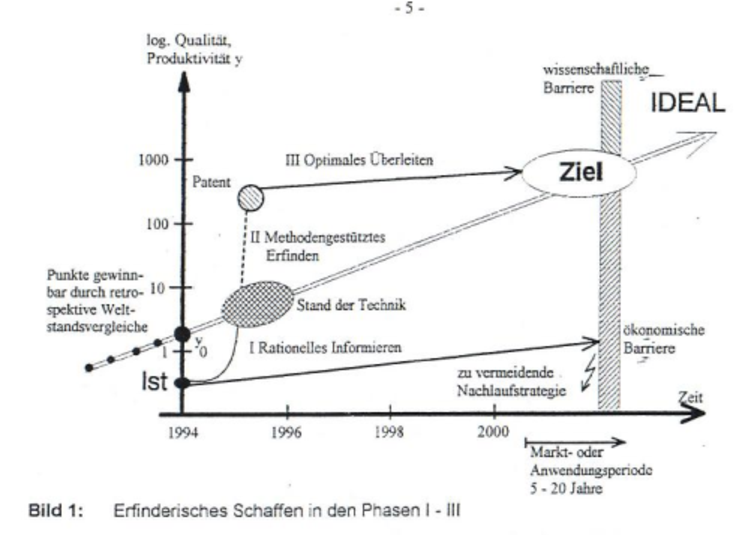
\includegraphics[width=.9\textwidth]{HF-B.pdf}
  
  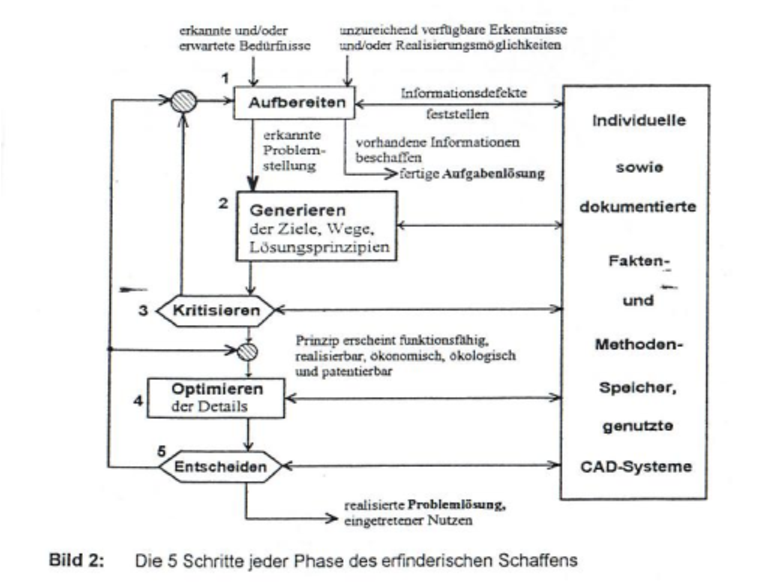
\includegraphics[width=.9\textwidth]{HF-C.pdf}
  \newpage
  
  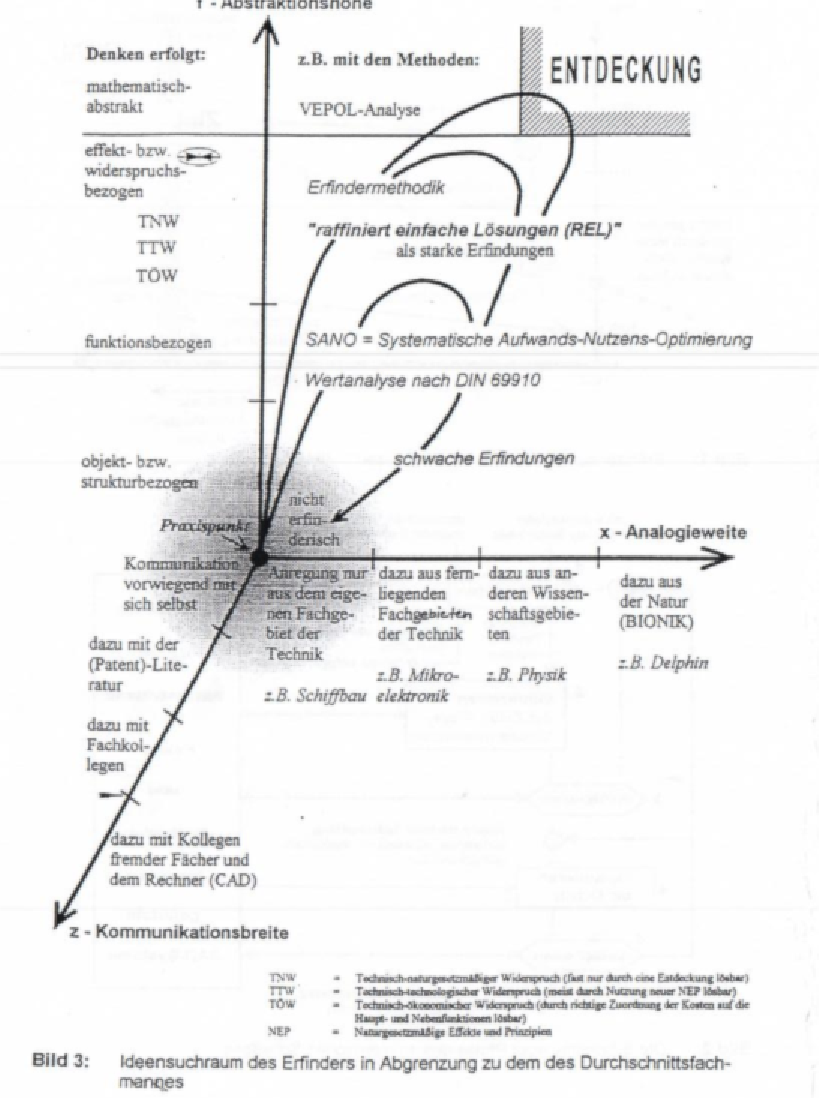
\includegraphics[width=.9\textwidth]{HF-A.pdf}
\end{center}
\newpage

\section*{5. Das Rationelle Informieren}

Der vorgegebene Rahmen würde gesprengt, wenn alle drei Phasen ausführlich
erläutert wür\-den.  Wenn Lerninteresse besteht, können jederzeit in Leipzig
oder anderswo die Seminare besucht werden.

Nur zwei Beispiele aus über 40 trainierten Arbeitsschwerpunkten:
\begin{itemize}
\item Viele Entwickler berücksichtigen die über die Internationale
  Patentklassifikation leicht, auch rechnergestützt, auswertbare
  Patentliteratur nicht und verschenken dadurch einen Großteil des
  vorhandenen, frei nutzbaren Weltwissens. Etwa 30\% der Forschungsmittel
  werden durch Parallelentwicklungen vergeudet.

  Wer nur deutsche Parentliteratur auswertet, erfasst nur etwa 8\% des
  Weltpatentfonds!
\item Wer gleich Patente in der Langfassung liest, vergeudet Zeit und kann
  ohnehin nicht aktuell informiert bleiben, da auf den Gebieten der
  Spitzentechnologien teilweise über 3\,000 Patenatmeleinen pro Woche
  international registriert werden. Rationeller ist es, systematisch die über
  den WILA-Verlag beziehbaren Kurzfassungen mit Hauptzeichnung der Patente zu
  verfolgen. Mit nur etwa 4\% Lesezeit kann eine über 80\%-ige
  Inhaltserschließung erfolgen. Ganz genau werden dann nur noch die drei bis
  zehn naheliegenden Schutzrechte analysiert.
\end{itemize}

\section*{6. Methoden- und rechnergestütztes Erfinden}

Mit den Methoden des \textbf{Zuspitzens der Forderungen}, der
\textbf{Schwachstellenanalyse} und des \textbf{historischen Herangehens}
werden die erfinderisch zu lösenden Widersprüche herausgearbeitet, welche in
der meist zu allgemeinen, ursprünglichen Problemstellung („Wir müssen
besser als die Konkurrenz  werden“ oder: "Unsere Qualität genügt nicht
mehr“ oder: „Der Absatz muss gesteigert; die Kosten gesenkt werden“) nicht
lösungsmotivierend formuliert sind.

Nun wird durch ein problembezogenes (Patent) Literaturstudium in der
Selbstarbeitsphase des Erfinderseminars nach Lösungesansätzen, vorwiegend
mittels der \textbf{Analogiemethode} gefahndet, wobei auch unser
PC-Expertensysten befragt werden kann.  Es nennt 260 erfinderisch nutzbare
naturgesetzmäßige Effekte und Prinzipien (NEP); der spontan arbeitende
Erfinder nutzt maximal 10!

Über 35 Erfindermethoden verhelfen dann meist schon nach einer Woche zum
erfinderischen Lösungsansatz.

Das \textbf{„Scheidungsprinzip“} führt durch Nutzung neuartiger NEP zu
raffiniert einfachen Lösungen (REL), weil die Technik nur noch zum
Optimieren der ansonsten kostenlosen und präzise arbeitenden NEP dient.

\emph{Beispiel:}

Um flüssige Pharmaka genau zu dosieren, müssen milligrammgenaue Mengen
bereitgestellt werden.  Präzisionswaagen sind sehr teuer.  Der erfinderische,
spottbillige Plastiktropfenbildner nutzt das konstante Verhältnis von
Oberflächenspannung sowie Masse und dosiert auf Milligramm genau.

Sollte keine Lösungsidee entstanden sein, wird das
\textbf{„Reißverschlussprinzip“} angewandt. Es empfiehlt das räumliche
und/oder zeitliche Trennen der Widerspruchspartner.

\emph{Beispiel:}

Um einen Nagel in Holz zu treiben, werden je nach Holzart teilweise über
1000\,MPa benötigt.  Eine entsprechende Presse wäre sehr teuer. Der
erfinderische Hammer löst das Problem einfach und preiswert, indem in mehreren
Schlägen Energie gesammelt und konzentriert auf den Nagel abgegeben wird.
Auch die Erfindermethode \textbf{„Mikrosystem“} führt oftmals zu „raffiniert
einfachen“ Lösungen.

\emph{Beispiel:}

Der objekthezogen denkende, nicht-erfinderische Mensch baut z.B. auch in
Kindergärten Türen mit Zapfen und Angel ein, obwohl am Spalt durch die
Hebelwirkung der Tür schwerste Quetschungen an Kinderhänden entstehen können.
Bei Taschen und zunehmend auch bei Koffern nutzt man erfinderisch die
Elastizität (Mirkoscharniere) spaltloser Gelenke; warum nicht auch bei Türen?

\section*{7. Optimales Überleiten}

Der Multierfinder Edison  soll das Erfinden definiert haben als
\begin{center}\bf  
  „1\% Intuition und  99\% Transpiration“.
\end{center}
Die Phasen 1 und 3 gehören zu Letzterem.

Ohne ein funktionsfähiges Referenzmuster vorführen zu können, gelingt fast
nie die erfolgreiche Vermarktung einer noch so guten Erfindung.

Das Materialisieren einer Erfindung erfordert aber meist viel Zeit und Geld.
Allem Neuen haften zwangsläufig Kinderkrankheiten an, die behoben werden
müssen; der Teufel steckt meist im Detail.  Trotz aller Motivation bleibt der
Erfinder meist auf der Strecke, wenn er nicht aktive Helfer und wohlwollende
Förderer findet.

Wer kennt sich z.B.  schon genau in den über 700 Förderprogrammen der EU, der
Bundes- oder Landesministerien aus?  Bei der Deutschen Erfinder-Akademie
können Ergänzungsseminare belegt werden, die Zugang zu Förderungen bis zu 800
TDM ermöglichen. Viele ehemalige Erfinderschüler nutzen diese Hilfen und haben
Innovationsunternehmen gegründet.

\section*{8. Zusammenfassung}

Erfinderisches Können ist nicht angeboren.  Es kann nach dem „Versuch und
Irrtum“-Prinzip autodidaktisch erworben werden.  Viel besser ist es aber, es
als geistigen „Hochleistungssport“ unter Anleitung erfahrener Trainer zu
erlernen.

Buchen Sie daher am besten mit einem Team schriftlich eines der nächsten
Zweitageseminare, werlche immer am Monatsende von Freitag, 11 Uhr bis
Sonnabend, 16 Uhr bei uns in Leipzig stattfinden und pro Person 600\,DM
kosten.  Schüler ab dem 16. Lebensjahr, Studenten, Arbeitslose und Rentner
zahlen nur die Hälfte. Sie können auch faxen 0341-6896149 und erhalten nach
Überweisung auf das u.g. Konto mit Angabe des Namens eine schrigftliche
Einladung oder Einweisung in das nächste Seminar, da nur in Kleingruppen
trainiert werden kann.

Wenn Sie die Seminare z.B. zusammen mit Unternehmen oder Instituten, dem VDI
oder RKW, mit der IHK oder HWK in Ihrem Heimatort selbst organisieren,
berechnen wir für ein Zweitageseminar pauschal 4\,000\,DM + MwSt. + Reise-
und Hotelspesen, so dass  Ihnen noch genügend Gewinn verbleibt.

%\ccnotice
\end{document}
